
% JuliaCon proceedings template
\documentclass{juliacon}
\setcounter{page}{1}

\begin{document}

% **************GENERATED FILE, DO NOT EDIT**************

\title{My JuliaCon proceeding}

\author[1]{1st author}
\author[1, 2]{2nd author}
\author[2]{3rd author}
\affil[1]{University}
\affil[2]{National Lab}

\keywords{Julia, Optimization, Game theory, Compiler}

\hypersetup{
pdftitle = {My JuliaCon proceeding},
pdfsubject = {JuliaCon 2019 Proceedings},
pdfauthor = {1st author, 2nd author, 3rd author},
pdfkeywords = {Julia, Optimization, Game theory, Compiler},
}



\maketitle

\begin{abstract}

MPI.jl is a Julia package for using the Message Passing Interface (MPI),
a standardized and widely-supported communication interface for
distributed computing, with multiple open source and proprietary
implementions. It roughly follows the C MPI interface, with some
additional conveniences afforded by the Julia language such as automatic
handling of buffer lengths and datatypes.

\end{abstract}

\section{Introduction}

Now over 25 years old, MPI is the stalwart of high-performance computing
communication, supported on everything from single machines to
billion-dollar supercomputers. Despite its age, it supports several
models of communication, and significant engineering effort goes into
optimizing performance and supporting the latest networking hardware.

Although Julia provides its own suite of distibuted computing tools via
the Distributed standard library, it is based on a controller/worker
model and is currently unable to leverage fast networking hardware such
as InfiniBand, which limits its scalability to large problems. MPI.jl
leverages the well-established and proven technology, including
extensions such as the CUDA-aware interfaces for multi-GPU
communication. It is being used by multiple Julia projects, including
the CliMA Earth system modelling project \cite{clima}.

\section{Simple example and running MPI programs}
\label{sec:simple-example}

Most MPI programs utilise a single-program, multiple-data (SPMD) model
where multiple processes all run the same program and communicate via
messages, with their data determined by the process rank (a 0-based
ordering of the processes).

An example of this is is a simple ``round-robin'' communication pattern
in which each process sends a message containing its rank to its next
neighbor using non-blocking point-to-point operations:

\begin{lstlisting}[language = Julia]
# sendrecv.jl
# initialize and set global variables
using MPI
MPI.Init()

comm = MPI.COMM_WORLD
rank = MPI.Comm_rank(comm)
N = MPI.Comm_size(comm)

# non-blocking receive from previous rank
recv_buf = Array{Float64}(undef, 2)
recv_req = MPI.Irecv!(recv_buf, mod(rank-1, N), 0,
                      comm)

# non-blocking send to next rank
send_buf = Float64[rank, rank]
send_req = MPI.Isend(send_buf, mod(rank+1, N), 0,
                     comm)

# block until communication is completed
MPI.Waitall!([recv_req, send_req])
print("$rank: Received $recv_buf\n")
\end{lstlisting}

This can be run using the MPI launcher (typically called
\verb mpiexec .

\begin{verbatim}
$ mpiexec -n 3 julia sendrecv.jl
0: Received [2.0, 2.0]
2: Received [1.0, 1.0]
1: Received [0.0, 0.0]
\end{verbatim}

\section{Implementation details and challenges}
\label{sec:implementation-details-and-challenges}

Although MPI.jl mirrors the C MPI interface quite closely, it does take
advantage of several features of the Julia language to improve
usability. The C and Fortran MPI interfaces require that users manually
check the error code returned by each function; MPI.jl is able to use
Julia's exception handling machinery to automatically check error codes
and print readable error messages. This allows functions to return their
results via return values instead of via additional functions arguments.
For example, non-blocking operations return \verb Request  objects;
blocking receive operations return their output buffers.

\subsection{Allocation and serialization}
\label{sec:allocation-and-serialization}

For communication operations which receive data, MPI.jl typically
defines two separate functions:

\begin{itemize}
\item
  one function in which the output buffer is supplied by the user: as it
  mutates this value, it adopts the Julia convention of suffixing with
  \verb !  (e.g.~\verb MPI.Recv! , \verb MPI.Reduce! ).
\item
  one function which allocates the buffer for the output
  (\verb MPI.Recv , \verb MPI.Reduce ).
\end{itemize}

Additionally, we adopt the convention from the mpi4py Python MPI
bindings \cite{dalcin2011parallel} of using lowercase names for
functions which are able to handle arbirary objects. These are typically
slower as they rely on serialization and are not type-stable, but can be
convenient as they don't require that the object type or size be known
by the receiver. Currently only a small number of these functions are
provided.

\subsection{Buffers, datatypes and operators}
\label{sec:buffers-datatypes-and-operators}

In C and Fortran, MPI communication functions require three arguments
(address, count and element datatype) to specify their input and/or
output buffers e.g.~the \verb MPI_Send  signature in C has six
arguments:
\begin{lstlisting}[language = C]
int MPI_Send(const void* buf, int count,
      MPI_Datatype datatype, int dest, int tag,
      MPI_Comm comm)
\end{lstlisting}

In Julia, these can all be determined from an \verb Array  object, so
the corresponding function in MPI.jl only requires 4 arguments:
\begin{lstlisting}[language = C]
MPI.Send(buf, dest::Integer, tag::Integer,
      comm::MPI.Comm)
\end{lstlisting}

An intermediate \verb Buffer  type is defined that captures the
necessary properties, and allows defining MPI communication operations
for other Julia objects without requiring that additional methods for
every communication function. For example, to support the CUDA-aware MPI
interface across all MPI functions, only a single additional
\verb Buffer(arr::CUDA.CuArray)  method was required.

If the element type of the buffer is not one of the predefined MPI
datatypes, then MPI.jl will automatically build and commit the
corresponding MPI user-defined type.

Similarly, for collective reduction operations (\verb MPI.Reduce ,
\verb MPI.Scan , etc.), MPI.jl will convert Julia functions to MPI
operator objects, either mapping to predefined operators
(e.g.~\verb +  to \verb MPI.SUM ), or wrapping functions to form
custom operators.

Both of these are illustrated in the pooled variance example in section \ref{sec:pooled-variance}.

\subsection{Application binary interface}
\label{sec:application-binary-interface}

The MPI standard specifies C and Fortran appilication programming
interfaces (API), but not an application binary interface (ABI).
Consequently, datatypes and enum values vary between different
implementations, and require parsing C headers to extract their precise
values. We use two approaches to work around this problem:

\begin{itemize}
\item
  Attempt to identify the MPI implementation by querying
  \verb MPI_Get_library_version , and use predefined constants and
  types if known to be compatible with MPICH, Open MPI or Microsoft MPI.
\item
  Otherwise, at build time it compiles a small C program that outputs
  the type sizes and constants. One complication is that the opaque C
  handles might only be defined at link time: in this case, we convert
  to the Fortran handle values (which are required to be integers), and
  convert back to C handles when calling \verb MPI.Init() . A similar
  approach is used by the MPI bindings for Rust \cite{rsmpi}.
\end{itemize}

\subsection{Binary support}
\label{sec:binary-support}

Similar to many Julia packages, MPI.jl uses BinaryBuilder and the
Artifacts system to automatically install an MPI implementation when the
package is installed (currently Microsoft MPI on Windows, MPICH on other
platforms), which simplifies the installation procedure for users on
single machines.

On high-performance computing systems one would typically want to use
system or other externally-provided binaries. To aid this, MPI.jl
provides additional hooks to enable switching this at build time via
environment variables, and a warning is show if a user appears to be
using the default MPI binary on a HPC system. Challenges remain on how
to make it easier to switch implementations (when multiple are present),
or how to deal with binaries which depend on MPI.


\section{Examples}
\label{sec:examples}

\subsection{Ping pong benchmark}
\label{sec:ping-pong-benchmark}

The ``ping pong'' benchmark consists of two MPI processes which
alternate sending messages between each other, and is a useful measure
of how function call overhead affects communication latency.

A simple Julia implementation is:
\begin{lstlisting}[language = Julia]
function pingpong(T, bufsize, iters)
    buffer = zeros(T, bufsize)
    comm = MPI.COMM_WORLD
    rank = MPI.Comm_rank(comm)
    tag = 0

    MPI.Barrier(MPI.COMM_WORLD)
    tic = MPI.Wtime()
    for i = 1:iters
        if rank == 0
            MPI.Send(buffer, 1, tag, comm)
            MPI.Recv!(buffer, 1, tag, comm)
        else
            MPI.Recv!(buffer, 0, tag, comm)
            MPI.Send(buffer, 0, tag, comm)
        end
    end
    toc = MPI.Wtime()

    avgtime = (toc-tic)/iters
    return avgtime
end
\end{lstlisting}


\begin{figure}[t]
\centerline{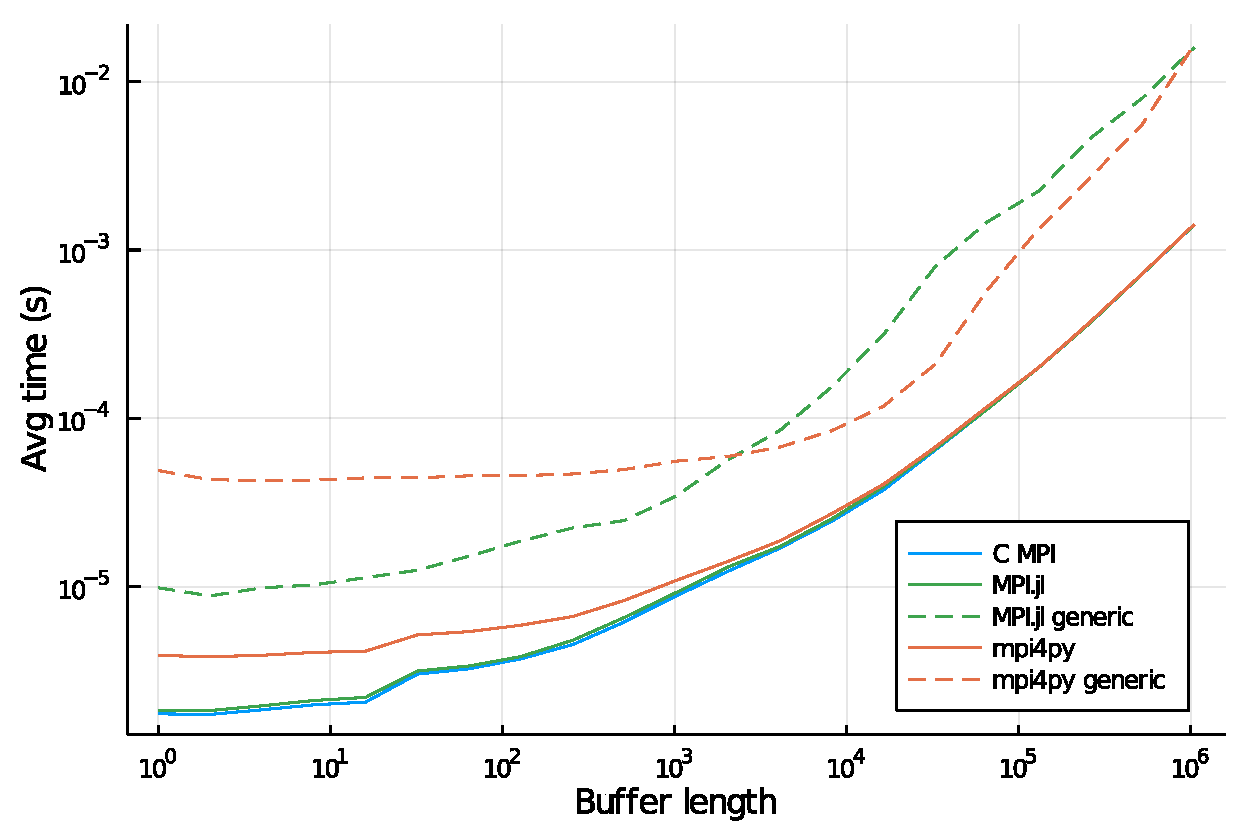
\includegraphics[width=0.5\textwidth]{pingpong.pdf}}
\caption{MPI ping pong benchmark in C, Julia (MPI.jl) and Python
(mpi4py) using arrays of 64-bit floating-point numbers. Benchmarks were
performed using Open MPI 4.0.4, using two processes on different nodes
connected by EDR InfiniBand.\label{fig:pingpong}}
\end{figure}

Figure \ref{fig:pingpong} compares the ping pong benchmark implemented in
C, Julia using MPI.jl, and Python using mpi4py. The MPI.jl benchmark
exhibits similar performance to C, whereas mpi4py is notable slower for
smaller message sizes, likely due to the intepreter overhead of Python.

In addition, for MPI.jl and mpi4py we also compare the lowercase
``generic'' \verb MPI.send and \verb MPI.recv  functions, which are able to
handle arbitrary objects. Here MPI.jl is still faster than mpi4py for
small messages, but slower for medium-sized messages. We suspect this is
due to garbage collection pauses in the Julia runtime.

\subsection{Minimum-spanning tree broadcast}
\label{sec:minimum-spanning-tree-broadcast}

Julia syntax is close to pseudo-code found in the literature to describe
parallel algorithms. For example, consider the minimum-spanning tree
broadcast algorithm in Figure 3a of \cite{chan2007collective}. A Julia
implementation is given as:

\begin{lstlisting}[language = Julia]
function MSTBcast(x, root, left, right, comm)
    me = MPI.Comm_rank(comm)
    tag = 999

    if left == right
        return x
    end
    mid = div((left + right),  2)
    dest = root <= mid ? right : left

    if me == root
        MPI.send(x, dest, tag, comm)
    end
    if me == dest
        (x, _) = MPI.recv(root, tag, comm)
    end

    if me <= mid && root <= mid
        MSTBcast(x, root, left, mid, comm)
    elseif me <= mid && root > mid
        MSTBcast(x, dest, left, mid, comm)
    elseif me > mid && root <= mid
        MSTBcast(x, dest, mid + 1, right, comm)
    elseif me > mid && root > mid
        MSTBcast(x, root, mid + 1, right, comm)
    end
end
\end{lstlisting}

This is nearly identical to the pseudo-code and can be called for all of
the datatypes supported by \verb MPI.send  and \verb MPI.recv , for
example arrays, functions, and dictionaries.

\subsection{Pooled variance using custom datatypes and operators}
\label{sec:pooled-variance}

The following example uses both custom MPI datatypes and custom
reduction operators to compute the pooled variance of a distributed
dataset in a numerically stable way, using a single communication
operation:

\begin{lstlisting}[language = Julia]
# Custom struct containing the summary statistics
# (mean, variance, count)
struct SummaryStat
    mean::Float64
    var::Float64
    n::Float64
end

function SummaryStat(X::AbstractArray)
    m = mean(X)
    v = varm(X,m, corrected=false)
    n = length(X)
    SummaryStat(m,v,n)
end

# Custom reduction operator, computing pooled mean,
# variance and length
function pool(S1::SummaryStat, S2::SummaryStat)
    n = S1.n + S2.n
    m = (S1.mean*S1.n + S2.mean*S2.n) / n
    v = (S1.n * (S1.var + S1.mean * (S1.mean-m)) +
         S2.n * (S2.var + S2.mean * (S2.mean-m)))/n
    SummaryStat(m,v,n)
end

# Perform a scalar reduction to `root`
summ = MPI.Reduce(SummaryStat(X), pool, root, comm)
\end{lstlisting}

\section{Acknowledgements}
\label{sec:acknowledgements}

We thank the many contributors to MPI.jl over the years: Erik Schnetter,
Jared Crean, Jake Bolewski, Davide Lasagna, Katharine Hyatt, Jeremy
Kozdon, Andreas Noack, Bart Janssens, Amit Murthy, Steven G. Johnson,
David Anthoff, Thomas Bolemann, Joey Huchette, Seyoon Ko, Juan Ignacio
Polanco, Tristan Konolige, Samuel Omlin, Mosè Giordano, Filippo
Vicentini, Keno Fischer, Maurizio Tomasi, Yuichi Motoyama, Tom Abel,
Jane Herriman, Ernesto Vargas, Elliot Saba, Rohan McLure, Randy Lai,
Mike Nolta, Josh Milthorpe, Michel Schanen, Kiran Pamnany, Joaquim Dias
Garcia, Jonathan Goldfarb, Chris Hill, Balazs Nemeth, Alberto F. Martin,
Ali Ramadhan, Viral Shah, Sacha Verweij, Kristoffer Carlsson, Joel Mason
and Yao Lu.

This research was made possible by the generosity of Eric and Wendy
Schmidt by recommendation of the Schmidt Futures program, Mountain
Philanthropies, the Paul G. Allen Family Foundation, and the National
Science Foundation (NSF award AGS-1835860).

\bibliographystyle{juliacon}
\bibliography{paper}

\end{document}

% Inspired by the International Journal of Computer Applications template
